%%%%%%% ICML 2018 EXAMPLE LATEX SUBMISSION FILE %%%%%%%%%%%%%%%%%

\documentclass{article}

% Recommended, but optional, packages for figures and better typesetting:
\usepackage{microtype}
\usepackage{graphicx}
\usepackage{subfigure}
\usepackage{booktabs} % for professional tables
\usepackage{enumitem}

\usepackage{bussproofs}

\usepackage{algpseudocode}
\usepackage{algorithmicx}
\usepackage{sourcecodepro}
\usepackage{listings}
\usepackage{amsfonts}
\usepackage{amssymb}
\usepackage{tikz-qtree}
\usepackage{amsthm}
\usepackage{bm}
\usetikzlibrary{bayesnet}
\usetikzlibrary{arrows}
\usepackage{caption}
\usepackage{subcaption}
\usetikzlibrary{backgrounds}

\newcommand{\E}{\mathbb{E}}
\newcommand{\Var}{\mathrm{Var}}
\newcommand{\Cov}{\mathrm{Cov}}

\usepackage{mathtools}% superior to amsmath
\usepackage{tikz}
\tikzset{latent/.append style={minimum size=14pt, inner sep=1pt, node distance=10pt}, every node/.append style={draw,circle, inner sep=1pt}}
\makeatletter
\newcommand\ccirc[1]{%
\mathpalette\@ccirc{#1}%
}
\newcommand\@ccirc[2]{%
\tikz[baseline=(math.base)] \node (math) {$\m@th#1#2$};%
}
\newcommand\gcirc[1]{%
\mathpalette\@gcirc{#1}%
}
\newcommand\@gcirc[2]{%
\tikz[baseline=(math.base)] \node[fill=gray!30] (math) {$\m@th#1#2$};%
}
\makeatother


% hyperref makes hyperlinks in the resulting PDF.
% If your build breaks (sometimes temporarily if a hyperlink spans a page)
% please comment out the following usepackage line and replace
% \usepackage{icml2018} with \usepackage[nohyperref]{icml2018} above.
\usepackage{hyperref}

% Attempt to make hyperref and algorithmic work together better:
\newcommand{\theHalgorithm}{\arabic{algorithm}}

% Use the following line for the initial blind version submitted for review:
%\usepackage{icml2018_ift6269}

% If accepted, instead use the following line for the camera-ready submission:
\usepackage[accepted]{icml2018_ift6269}
% SLJ: -> use this for your IFT 6269 project report!

\usepackage[skins,breakable,listings]{tcolorbox}

\lstset{basicstyle=\ttfamily,breaklines=true}
\usepackage{upquote}
%\def\backtick{\char18}
\lstdefinestyle{backtickstyle}{literate={`}{\char}1, escapechar=@}

\usepackage{fontspec}

\makeatletter
\def\verbatim@nolig@list{}
\makeatother

\setmonofont{JetBrains Mono}[Contextuals=Alternate]

\usepackage{ocr}
\usepackage[T1]{fontenc}

\usepackage{accsupp}
\newcommand{\noncopyable}[1]{%
\BeginAccSupp{method=escape,ActualText={}}%
#1%
\EndAccSupp{}%
}

\lstdefinelanguage{kotlin}{
comment=[l]{//},
commentstyle={\color{gray}\ttfamily},
emph={delegate, filter, firstOrNull, forEach, it, lazy, mapNotNull, println, repeat, assert, with, head, tail, len, return@},
numberstyle=\noncopyable,
emphstyle={\color{olive}},
identifierstyle=\color{black},
keywords={abstract, actual, as, as?, break, by, class, companion, continue, data, do, dynamic, else, enum, expect, false, final, for, fun, get, if, import, in, infix, interface, internal, is, null, object, open, operator, override, package, private, public, return, sealed, set, super, suspend, this, throw, true, try, catch, typealias, val, var, vararg, when, where, while, tailrec, reified, Repeat},
keywordstyle={\color{blue}\bfseries},
morecomment=[s]{/*}{*/},
morestring=[b]",
morestring=[s]{"""*}{*"""},
ndkeywords={@Deprecated, @JvmField, @JvmName, @JvmOverloads, @JvmStatic, @JvmSynthetic, Array, Byte, Double, Float, Boolean, Int, Integer, Iterable, Long, Runnable, Short, String, Pair, Gaussian},
ndkeywordstyle={\color{purple}\bfseries},
sensitive=true,
stringstyle={\color{green}\ttfamily},
literate={`}{{\char0}}1
}

\newtcblisting{kotlinlisting}[1][]{%
listing options={
language=kotlin,
basicstyle=\scriptsize\ttfamily,
%numberstyle=\footnotesize\noncopyable,
showstringspaces=false,
tabsize=2,
breaklines=true,
%numbers=right,
inputencoding=utf8,
escapeinside={(*@}{@*)},
#1
},
underlay unbroken and first={%
\path[draw=none] (interior.north west) rectangle node[white]{
\includegraphics[width=4mm]{kotlin_file.png}} ([xshift=-10mm,yshift=-12mm]interior.north west);
}
}

\tcbset{
enhanced jigsaw,
listing only,
%boxsep=-1pt,
%top=-1pt,
%bottom=-0.5pt,
center,
width=0.42\textwidth,
%right=-0.5pt,
overlay first={
\node[black!50] (S) at (frame.south) {\Large\ding{34}};
\draw[dashed,black!50] (frame.south west) -- (S) -- (frame.south east);
},
overlay middle={
\node[black!50] (S) at (frame.south) {\Large\ding{34}};
\draw[dashed,black!50] (frame.south west) -- (S) -- (frame.south east);
\node[black!50] (S) at (frame.north) {\Large\ding{34}};
\draw[dashed,black!50] (frame.north west) -- (S) -- (frame.north east);
},
overlay last={
\node[black!50] (S) at (frame.north) {\Large\ding{34}};
\draw[dashed,black!50] (frame.north west) -- (S) -- (frame.north east);
},
before={\par\vspace{5pt}},
after={\par\vspace{5pt}\noindent}
}

\newcommand*{\inlineimg}[1]{%
\raisebox{-.3\baselineskip}{%
\includegraphics[
height=\baselineskip,
width=\baselineskip,
keepaspectratio,
]{#1}%
}%
}

\definecolor{slightgray}{rgb}{0.90, 0.90, 0.90}

\usepackage{soul}
\usepackage{hyperref}
\makeatletter
\def\SOUL@hlpreamble{%
\setul{}{3.0ex}%
\let\SOUL@stcolor\SOUL@hlcolor%
\SOUL@stpreamble%
}
\makeatother

\newcommand{\inline}[1]{%
\begingroup%
\sethlcolor{slightgray}%
\hl{\ttfamily\footnotesize #1}%
\endgroup
}

\newcommand{\tinline}[1]{%
\begingroup%
\sethlcolor{slightgray}%
\hl{\ttfamily\tiny #1}%
\endgroup
}

% The \icmltitle you define below is probably too long as a header.
% Therefore, a short form for the running title is supplied here:
\icmltitlerunning{IFT 6269 Final Report: Probabilistic Reasoning, from Graphs to Circuits}

\begin{document}

\twocolumn[
\icmltitle{IFT 6269 Final Report: Probabilistic Reasoning, from Graphs to Circuits}

% It is OKAY to include author information, even for blind
% submissions: the style file will automatically remove it for you
% unless you've provided the [accepted] option to the icml2018
% package.

% List of affiliations: The first argument should be a (short)
% identifier you will use later to specify author affiliations
% Academic affiliations should list Department, University, City, Region, Country
% Industry affiliations should list Company, City, Region, Country

% You can specify symbols, otherwise they are numbered in order.
% Ideally, you should not use this facility. Affiliations will be numbered
% in order of appearance and this is the preferred way.
\icmlsetsymbol{equal}{*}

\begin{icmlauthorlist}
\icmlauthor{Breandan Considine}{socs,kast,mila}
\end{icmlauthorlist}

\icmlaffiliation{socs}{McGill University, School of Computer Science}
\icmlaffiliation{kast}{Knowledge and Software Technology Lab}
\icmlaffiliation{mila}{Mila Queb\'ec}

\icmlcorrespondingauthor{Breandan Considine}{breandan.considine@mail.mcgill.ca}

% You may provide any keywords that you
% find helpful for describing your paper; these are used to populate
% the "keywords" metadata in the PDF but will not be shown in the document
\icmlkeywords{Machine Learning, ICML}

\vskip 0.3in
]

% this must go after the closing bracket ] following \twocolumn[ ...

% This command actually creates the footnote in the first column
% listing the affiliations and the copyright notice.
% The command takes one argument, which is text to display at the start of the footnote.
% The \icmlEqualContribution command is standard text for equal contribution.
% Remove it (just {}) if you do not need this facility.

%\printAffiliationsAndNotice{}  % leave blank if no need to mention equal contribution
\printAffiliationsAndNotice{} % otherwise use the standard text.

\begin{abstract}
    Graphical models (PGMs) are very expressive, but even approximate inference on belief networks (BNs) is NP-hard~\citep{dagum1993approximating}. We can faithfully represent a large class of PGMs and their corresponding distributions as probabilistic circuits (PCs)~\citep{choi2020probabilistic}, which are capable of exact inference in polynomial time and tractable to calibrate using SGD or EM. PCs share many algebraic properties with PGMs and can propagate statistical estimators using simple algebraic rules. In this work, we will see how to compile BNs to PCs using the approach developed by \citet{zhao2015relationship}, and demonstrate their equivalence on a few toy inference problems.
\end{abstract}

\section{Introduction}\label{sec:intro}

Probabilistic inference is logical framework for reasoning about uncertainty. In this work, we define a denotational and operational semantics for probabilisic inference based on constructive logic, then build a \href{https://github.com/breandan/markovian}{concrete implementation} by translating those inference rules to the Kotlin language.

Let $E$ be a set of events and $S$ be a set of subsets of $E$. A \textit{probability distribution} is a function $P: S \rightarrow \mathbb{R}^{+}$ which satisfies the~\citet{kolmogorov1933grundbegriffe} axioms, in particular:

\begin{itemize}
    \itemsep-1em
    \item [(3)] $P(S = s) \in \mathbb{R}^{+}, \forall s \in S$.& \\
    \item [(4)] $P(E) = 1$. ($S = $ may be omitted for brevity.)& \\
    \item [(5)] $P(X \cup Y) = P(X) + P(Y), \forall X \cap Y = \varnothing$.
\end{itemize}

% https://math.stackexchange.com/questions/3573008/kolmogorov-probability-theory-question
% https://archive.org/details/foundationsofthe00kolm/page/2/mode/2up


%The simplest distribution assigns equal probability to all $\omega \in \Omega$. This is called the uniform distribution, $\mathcal{U}$.
%
%$$
%\mathcal U(\omega_1) = \mathcal U(\omega_2)\text{, } \forall \omega_1, \omega_2 \in \Omega
%$$

Some common exponential family distributions include:

\begin{tabular}{cccc}
    $\mathcal{D} \rightarrow \text{Gaussian}$ &
    $\mathcal{D} \rightarrow \text{Bernoulli}$ &
    $\mathcal{D} \rightarrow \text{Dirichlet}$ &
\end{tabular}

We can join two distributions to form a \textit{joint distribution}:

\begin{center}
\begin{tabular}{ccc}
    $\mathcal{D} \rightarrow \mathcal{D}, \mathcal{D}$ &$\mathcal{J} \rightarrow P(\mathcal{D})$ &$\mathcal{J} \rightarrow \mathcal{J}\mathcal{J}$
\end{tabular}
\end{center}

Given a distribution over a set $X$, we can \textit{sample} from it to produce a single element from that set, a \textit{random variable}:

\begin{prooftree}
    \AxiomC{$\Gamma \vdash P(X): X \rightarrow \mathbb{R}^{+}$}
    \AxiomC{$x \sim P(X)$}
    \RightLabel{Sample}
    \BinaryInfC{$\Gamma \vdash x: (X\rightarrow \mathbb{R}^{+}) \leadsto X$}
\end{prooftree}

%We can assign a probability distribution to a variable, by \textit{sampling} from it. As we increase the sample size, the distribution of values will converge to the true distribution.
%
%$$
%d \sim \mathcal{D}
%$$

The joint distribution $P(X, Y)$ is a distribution over the Cartesian product of the sets $X$ and $Y$, denoted $X \times Y$:

\begin{prooftree}
    \AxiomC{$\Gamma \vdash P(X): X \rightarrow \mathbb R^{+}$}
    \AxiomC{$\Gamma \vdash P(Y): Y \rightarrow \mathbb R^{+}$}
    \RightLabel{Joint}
    \BinaryInfC{$\Gamma \vdash P(X, Y): X \times Y \rightarrow \mathbb R^{+}$}
\end{prooftree}

Given a joint distribution $P(X, Y)$, if we see an event $y: Y$, this observation is called \textit{conditioning} and the resulting distribution over $X$ is called a \textit{conditional distribution}:

% https://www.cambridge.org/core/services/aop-cambridge-core/content/view/819623B1B5B33836476618AC0621F0EE/9781108488518AR.pdf/Foundations_of_Probabilistic_Programming.pdf?event-type=FTLA#page=325

\begin{prooftree}
    \AxiomC{$\Gamma \vdash P(X, Y): X \times Y\rightarrow\mathbb{R}^+$}
    \AxiomC{$\Gamma \vdash y: Y$}
    \RightLabel{Cond}
    \BinaryInfC{$\Gamma \vdash P(X \mid Y = y): X\rightarrow\mathbb{R}^+$}
\end{prooftree}


Given a conditional distribution and its prior, to exchange the order of conditioning, we can use \citet{bayes1763essay} rule:

\begin{prooftree}
    \AxiomC{$P(X \mid Y)$}
    \AxiomC{$P(Y)$}
    \RightLabel{Bayes}
    \BinaryInfC{$P(Y \mid X) \propto P(X \mid Y)P(Y)$}
\end{prooftree}

When a conditional distribution $P(X \mid Y)$ does not depend on its prior $Y$, $X$ and $Y$ are called \textit{independent}.

\begin{prooftree}
    \AxiomC{$P(X \mid Y) = P(X)$}
    \RightLabel{Ind}
    \UnaryInfC{$X \perp Y$}
\end{prooftree}


Equivalently, when two distributions $P(X)$ and $P(Y)$ are multiplied to form a joint distribution $P(X, Y)$, we may conclude that $X$ and $Y$ are independent:

\begin{prooftree}
    \AxiomC{$P(X, Y) = P(X)P(Y)$}
    \RightLabel{Fact}
    \UnaryInfC{$X \perp Y$}
\end{prooftree}

When two conditionals $P(X \mid Z)$, $P(Y \mid Z)$ are multiplied to form a joint distribution $P(X, Y \mid Z)$, $X$ and $Y$ are said to be \textit{conditionally independent given $Z$}:

\begin{prooftree}
    \AxiomC{$P(X,Y \mid Z) = P(X \mid Z)P(Y \mid Z)$}
    \RightLabel{CondInd}
    \UnaryInfC{$X \perp Y \mid Z$ }
\end{prooftree}

%To draw a single sample from a distribution $\mathcal{D}$, we can do so as follows:
%
%$$
%
%$$

\section{Operational Semantics}

So far, we have defined the denotational semantics of probabilities. But what about the operational semantics?

To sample efficiently, we need to draw a sample from a uniform distribution (PRNG) and push it through some kind of function. But what function should we use to ensure samples converge to a given PDF in the limit? Unfortunately, such function does not exist in closed form for most distributions. We can only describe it indirectly.

% https://en.wikipedia.org/wiki/Inverse_transform_sampling

\begin{prooftree}
    \AxiomC{$x \sim P(X)$}
    \AxiomC{$\texttt{CDF}: x \mapsto \int P(X = x)dx$}
    \RightLabel{Draw}
    \BinaryInfC{$x = \texttt{INV(CDF(PRNG()))}$}
\end{prooftree}

If we have two distributions, how can we combine them to obtain numerical values? There are various ways to combine probability distributions. For independent random variables, the joint distribution is simply the product of their distributions:

% https://en.wikipedia.org/wiki/Joint_probability_distribution#Joint_distribution_for_independent_variables

\begin{prooftree}
    \AxiomC{$P(X)$}
    \AxiomC{$P(Y)$}
    \RightLabel{Join}
    \BinaryInfC{$P(X, Y) = P(X)P(Y)$}
\end{prooftree}

For dependent random variables, we need to know the dependence structure. Suppose we knew they were related by a mathematical formula. All mathematical formulae can be described as compositions of a few elementary operators.

The sum of two distributions is \textit{not} equivalent to the sum of their random variables. For independent random variables $X$ and $Y$, their sum is defined as convolution (\S~\ref{sec:combinators}) on the associated density functions:

% https://en.wikipedia.org/wiki/Convolution_of_probability_distributions#Introduction

\begin{prooftree}
    \AxiomC{$P(X)$}
    \AxiomC{$P(Y)$}
    \RightLabel{Conv}
    \BinaryInfC{$P(X + Y) = P(X) * P(Y)$}
\end{prooftree}

Specifically, if $x, y$ are drawn from independent Gaussians:

% https://en.wikipedia.org/wiki/Sum_of_normally_distributed_random_variables#Independent_random_variables

\begin{prooftree}
    \AxiomC{$x \sim \mathcal{N}(\mu_x, \sigma^2_x)$}
    \AxiomC{$y \sim \mathcal{N}(\mu_y, \sigma^2_y)$}
    \AxiomC{$z = x + y$}
    \TrinaryInfC{$z \sim \mathcal{N}(\mu_x + \mu_y, \sigma^2_x + \sigma^2_x)$}
\end{prooftree}

Likewise, their product can be defined as an integral:

% https://en.wikipedia.org/wiki/Product_distribution#Derivation_for_independent_random_variables

\begin{prooftree}
    \AxiomC{$x \sim P(X)$}
    \AxiomC{$y \sim P(Y)$}
    \AxiomC{$z = xy$}
    \RightLabel{Conv}
    \TrinaryInfC{$P(Z = z) = \int P(X = x)P(Y=\frac{z}{x})\frac{1}{|x|}dx$}
\end{prooftree}

To remove a dimension from a joint distribution $P(X, Y)$ we can \textit{marginalize}, or sum over all possible conditionals. The resulting distribution is called a \textit{marginal distribution}:

\begin{prooftree}
    \AxiomC{$\Gamma \vdash P(X, Y): X\times Y\rightarrow\mathbb{R}^+$}
    \RightLabel{Margin}
    \UnaryInfC{$\Gamma \vdash P(X) \propto \sum_{y \in Y} P(X \mid Y = y)$}
\end{prooftree}


\pagebreak\section{Probabilistic Graphical Models}

Probabilistic graphical models~\citep{jordan2003introduction,koller2009probabilistic} (PGMs) are a framework for probabilistic inference on distributions whose conditional dependence structure may be expressed as a graph. The graph's edges capture conditional independence relations between RVs. One type of PGM is a directed graphical model (DGM).

If we observe a variable with two latent variables which are not conditionally independent, we call this a \textit{collider}.

% http://maximustann.github.io/mach/2015/07/06/belief-network-2/
% http://frnsys.com/notes/ai/foundations/probabilistic_graphical_models.html
\begin{prooftree}
    \AxiomC{$X \not\perp Y \mid Z$}
    \RightLabel{Collide}
    \UnaryInfC{
    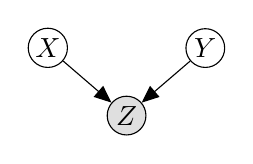
\begin{tikzpicture}
        \node[obs] (z) {$Z$};%
        \node[latent,above=of z,xshift=-1cm,fill] (x) {$X$}; %
        \node[latent,above=of z,xshift=1cm] (y) {$Y$}; %
        \edge {x,y} {z}
    \end{tikzpicture}
    }
\end{prooftree}

If we observe a variable with conditionally independent latent variables, we call this a \textit{fork} or equivalently, a \textit{chain}.

\begin{prooftree}
    \AxiomC{$X \perp Y \mid Z$}
    \RightLabel{Fork}
    \UnaryInfC{
    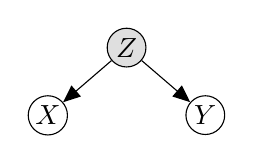
\begin{tikzpicture}
        \node[obs] (z) {$Z$};%
        \node[latent,below=of z,xshift=-1cm,fill] (x) {$X$}; %
        \node[latent,below=of z,xshift=1cm] (y) {$Y$}; %
        \edge {z} {x,y}
    \end{tikzpicture}
    }
    \DisplayProof
    \AxiomC{$X \perp Y \mid Z$}
    \RightLabel{Chain}
    \UnaryInfC{
    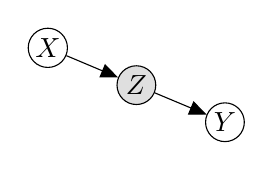
\begin{tikzpicture}
        \node[obs] (z) {$Z$};%
        \node[latent,above=of z,yshift=-11pt, xshift=-32pt,fill] (x) {$X$}; %
        \node[latent,below=of z,yshift=11pt, xshift=32pt] (y) {$Y$}; %
        \edge {x} {z}
        \edge {z} {y}
    \end{tikzpicture}
    }
\end{prooftree}

A belief network (BN) is an acyclic DGM of the form:

\begin{equation}
    P(x_1,\ldots,x_D)=\prod_{i=1}^D P(x_i \mid \texttt{parents}(x_i))
\end{equation}

% TODO: Variable elimination as graph transformation
% https://cedar.buffalo.edu/~srihari/CSE674/Chap9/9.3-VE-Algorithm.pdf#page=24
% https://www.youtube.com/watch?v=FDNB0A61PGE

\section{Probabilistic Circuits}\label{sec:language}

By defining some elementary distributions and composing them by means of simple operators, we obtain a rich framework for probabilistic modeling. Recent work~\citep{choi2020probabilistic} has explored tractable models for probabilistic reasoning based on semiring algebras. Semirings are known to have many useful applications in graph theory~\citep{dolan2013fun} and formal languages~\citep{bernady2013efficient}.

A semiring algebra has two operators, $\oplus$ and $\otimes$, with the usual properties. In particular, distributivity holds:

\begin{prooftree}
    \AxiomC{$X \otimes (Y \oplus Z)$}
    \UnaryInfC{$(X \otimes Y) \oplus (X \otimes Z)$}
    \DisplayProof
    \AxiomC{$(Y \oplus Z) \otimes X$}
    \RightLabel{Distrib}
    \UnaryInfC{$(X \otimes Y) \oplus (X \otimes Z)$}
\end{prooftree}

The sum product network (SPN) is a commutative semiring over univariate distributions~\citep{friesen2016sum}:

\begin{center}
    \begin{tabular}{ccc}
        $PC \rightarrow v \sim \mathcal{D}$ &
        $PC \rightarrow PC \oplus PC$ &
        $PC \rightarrow PC \otimes PC$
    \end{tabular}
\end{center}

Given a BN, we can compile it to a SPN using the procedure described by~\citet{butz2019sum}:

% Topsort: https://epubs.siam.org/doi/pdf/10.1137/0210049#page=17

\begin{algorithm}[H]
\caption{Bayes Network to Sum-Product Network}
\begin{algorithmic}[1]
\Procedure{BayesNetToSPN}{$bn$: BN}: SPN
\State $ac \leftarrow $\Call{VariableEliminate}{$bn$}
\State $ac \leftarrow $\Call{RedistributeParameters}{$ac$}
\State $ac \leftarrow $\Call{CompileMarginalized}{$ac$}
\State \Return{\Call{ReduceCircuit}{$ac$}}
\EndProcedure\\
\Procedure{ReduceCircuit}{$ac_0$: AC}: SPN
\State $ac_1 \leftarrow $ \Call{AddTerminalNodes}{$ac_0$}
\State $ac_1 \leftarrow $ \Call{MergeProducts}{$ac_1$}
\If{$ac_0 = ac_1$}
\State \Return{$ac_0$}
\Else
\State \Return{\Call{ReduceCircuit}{$ac_1$}}
\EndIf
\EndProcedure
\end{algorithmic}
\end{algorithm}

\section{DSL}

Our DSL implements these rules for Gaussian SPNs.

\begin{kotlinlisting}
val g0 = Gaussian(mu = 0.1,  sigma = 1.0)
val g1 = Gaussian(mu = 5.0,  sigma = 1.0)
val g2 = Gaussian(mu = 10.0, sigma = 1.0)
val g3 = Gaussian(mu = 5.0,  sigma = 2.0)
val g4 = g0 + g1 + g2
val g5 = g3 * g4
compare(g0, g1, g2, g3, g4, g5).display()
\end{kotlinlisting}

This program produces the following image when run:

\begin{figure}[h]
    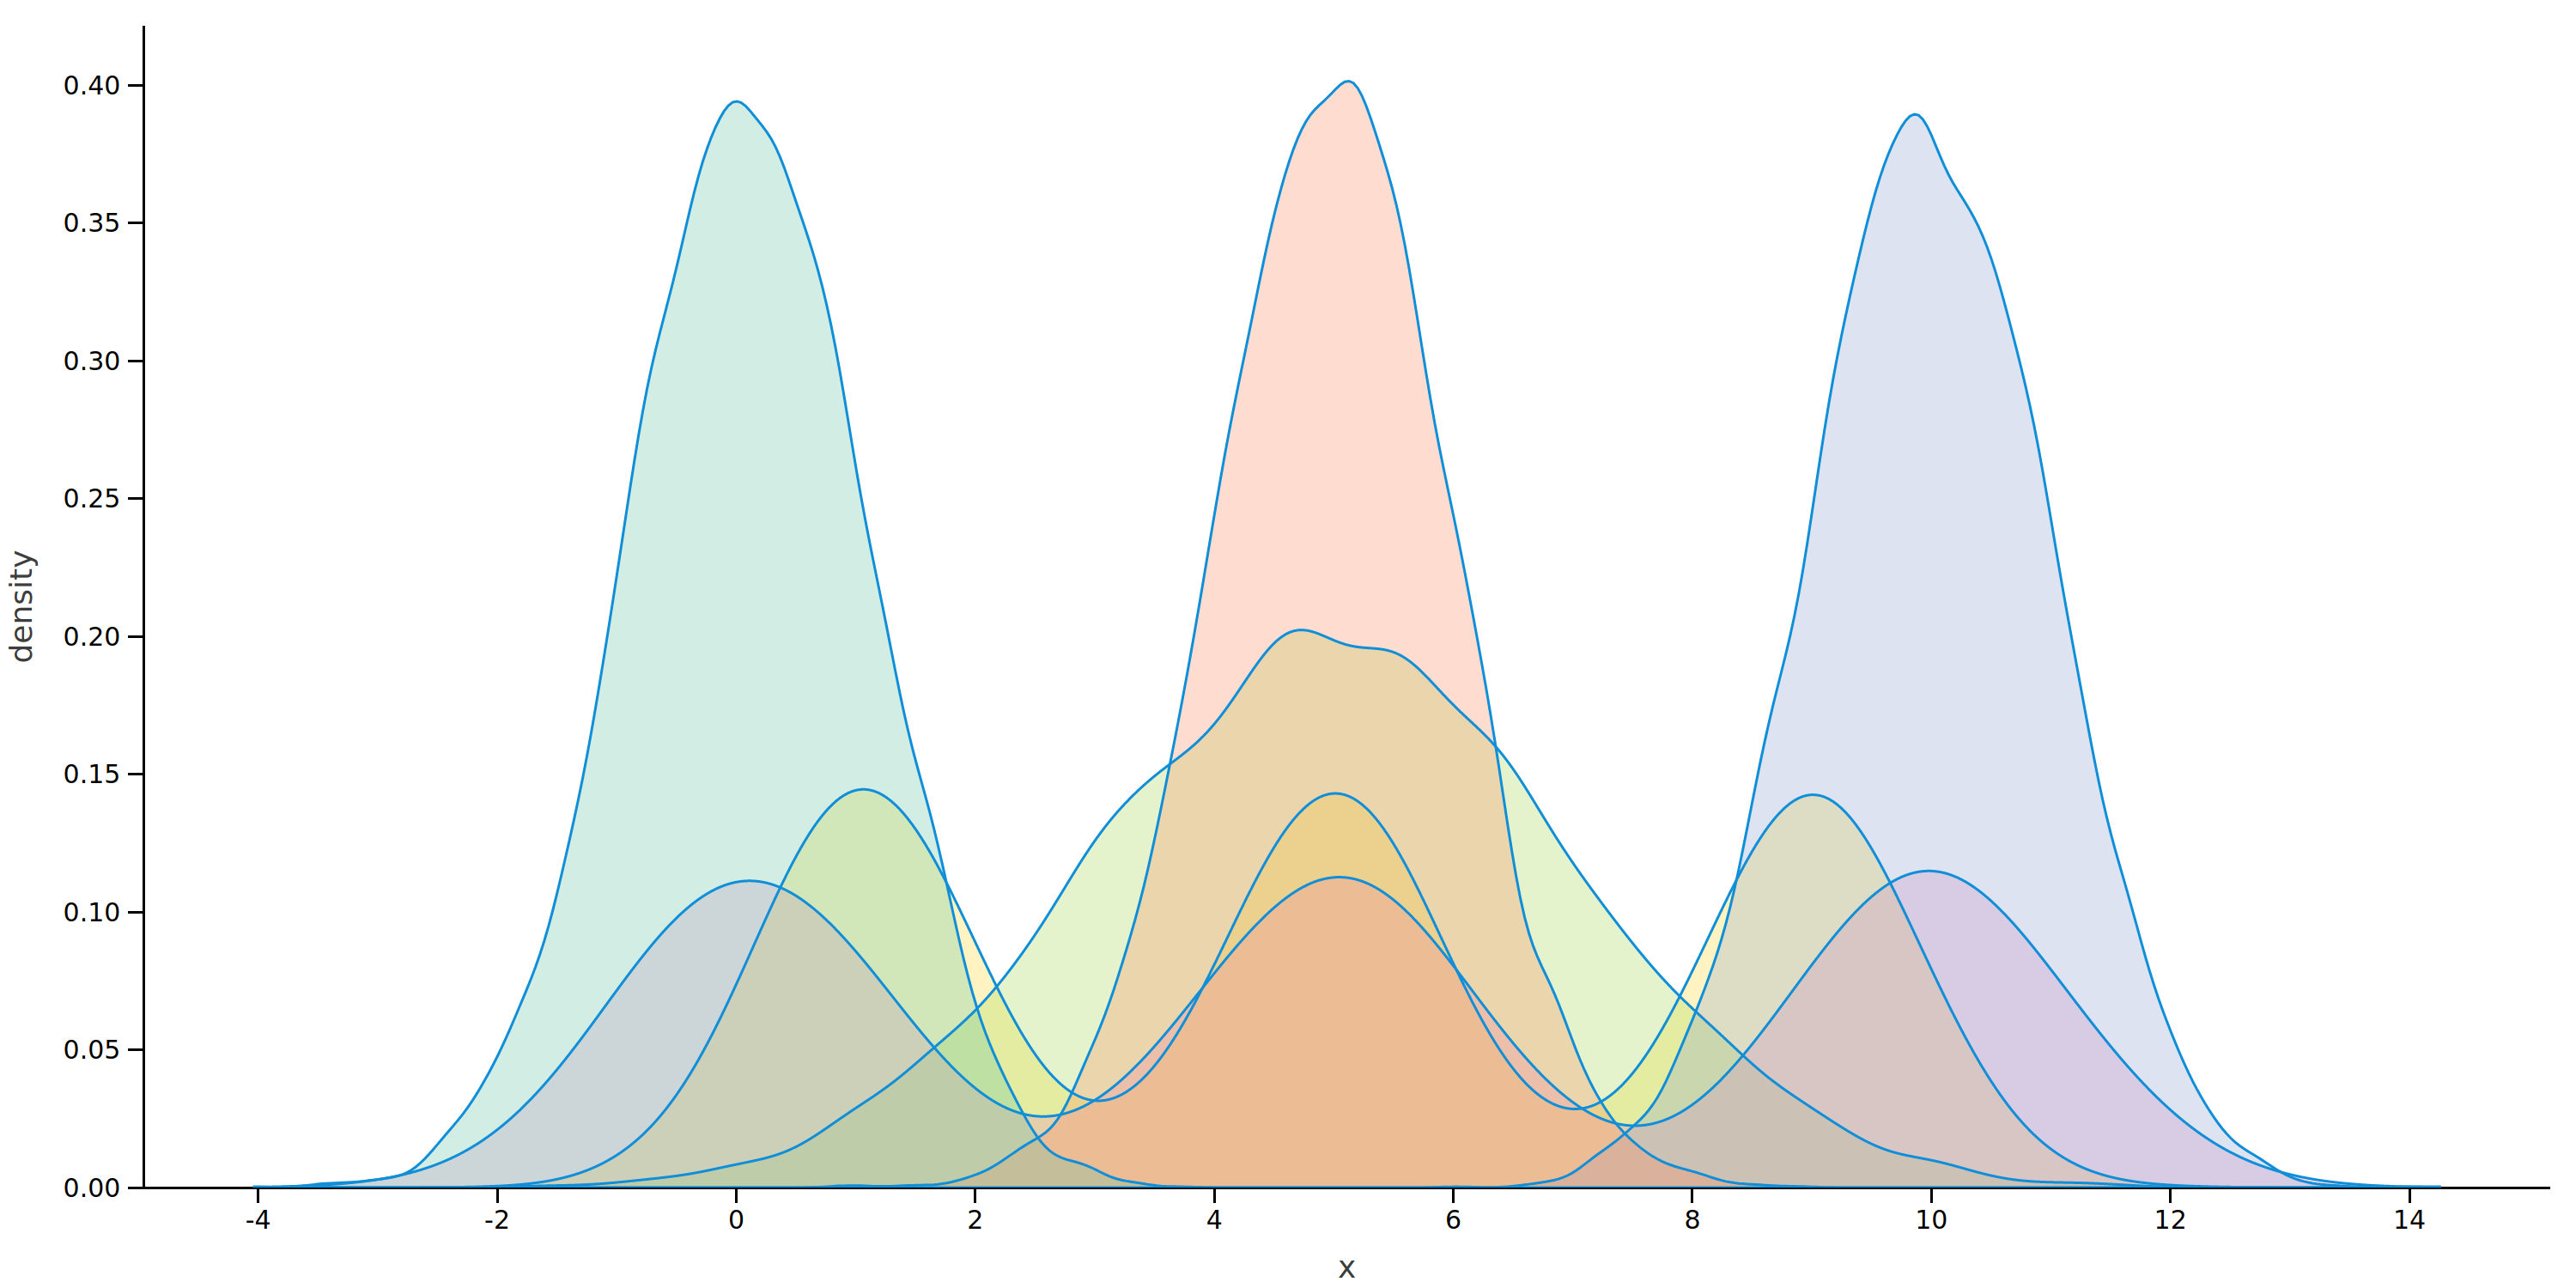
\includegraphics[width=0.4\textwidth]{plot.png}
    \centering
    \caption{10k samples from the SPN defined above.}
\end{figure}

%Our implementation is available at the following URL: \url{https://github.com/breandan/markovian}


\section{Inference}

EVI, MAR, CON, MAP, KLD inference is computationally tractable~\citep{choi2020probabilistic}. (TODO)

\section{Learning}

The strucutre of SPNs can be learned using the algorithm proposed by~\citet{gens2013learning}. (TODO)


\section{Conclusion}

Prior work~\citep{considine2019kotlingrad,considine2019programming} explored differentiable programming. Differentiability plays a key role in learning, but does not provide the necessary vocabulary to describe human knowledge. In order to capture human knowledge and begin to reason as humans do, programs must be able to express \textit{uncertainty}.

What is the probability of observing local variations? How are those observations related? And how do local variations affect global behavior? In order to correctly pose these questions and begin to answer them, we must be able to reason about uncertainty~\citep{pearl2014probabilistic}. In order to do so, we first defined some relations between probability distributions. We showed how to rewrite and factorize them in various contexts, and sample from them programmatically.

Graphs are a natural representation for both programs~\citep{allamanis2017learning} and probabilistic models~\citep{pearl2014probabilistic}. The language of linear algebra provides a unifying framework for many graph algorithms and computational tasks~\citep{kepner2011graph}. Recent evidence suggests probabilisitic inference is tractable for a large class of graphical models~\citep{choi2020probabilistic}. And sparse matrix representations enable efficient execution of large graphs on modern graphics processors~\citep{kepner2016mathematical}.

In future work, we will show how to learn a BN from data, compare its performance with BNs using a toy dataset and show that inference is empirically tractable.
\bibliography{example_paper}
\bibliographystyle{icml2018}


\section{Appendix}\label{sec:appendix}

\subsection{Combinators}\label{sec:combinators}

The \textit{convolution} operator $*$ is defined as the sum of a product at each point:

\begin{prooftree}
    \AxiomC{$\Gamma \vdash g: S^d \rightarrow \mathbb{R}, h: S^d \rightarrow \mathbb R$}
    \RightLabel{DiscConv}
    \UnaryInfC{$(g * h)(x) = \int_{\mathbb R^d} f(y)g(x - y)dy$}
    \DisplayProof

    \AxiomC{$\Gamma \vdash g: S^d \rightarrow \mathbb{Z}, h: S^d \rightarrow \mathbb Z$}
    \RightLabel{ContConv}
    \UnaryInfC{$(g * h)(x) = \sum_{\mathbb R^d} f(y)g(x - y)$}
\end{prooftree}

\subsection{Formal Language}

We can derive closed form estimators for SPNs, including expectation and variance, using the following formulae:

% https://en.wikipedia.org/wiki/Propagation_of_uncertainty

\begin{prooftree}
    \AxiomC{$\Gamma \vdash A: \mathcal D, B: \mathcal D$}
    \AxiomC{$C = A + B$}
    \RightLabel{VSum}
    \BinaryInfC{$\Var[C]^2 = \sqrt{\Var[A]^2 + \Var[B]^2 + 2\cdot\Cov[A, B]}$}
    \DisplayProof

    \AxiomC{$\Gamma \vdash A: \mathcal D, B: \mathcal D$}
    \AxiomC{$C = AB$}
    \RightLabel{VProd}
    \BinaryInfC{$\Var[C]^2 = C\sqrt{\frac{\Var[A]^2}{A^2} + \frac{\Var[B]^2}{B^2} + 2\frac{\Cov[A, B]}{AB}}$}
    \DisplayProof


    \AxiomC{$\Gamma \vdash A: \mathcal D, B: \mathcal D$}
    \AxiomC{$C = A + B$}
    \RightLabel{ESum}
    \BinaryInfC{$\E[C] = \E[A] + \E[B]$}
    \DisplayProof

    \AxiomC{$\Gamma \vdash A: \mathcal D, B: \mathcal D$}
    \AxiomC{$C = AB$}
    \RightLabel{EProd (IID)}
    \BinaryInfC{$\E[C] = \E[A]\E[B]$}
\end{prooftree}

\subsection{Probabilistic Graphical Models}

Following \citet{pearl1985graphoids}, the grammar of conditional independence statements has some equivalence relations:

% http://ftp.cs.ucla.edu/pub/stat_ser/r53-L.pdf#page=8

\begin{prooftree}
    \AxiomC{$X \perp Y \mid Z$}
    \RightLabel{Sym}
    \UnaryInfC{$Y \perp X \mid Z$}
    \DisplayProof
    \hskip 1.5em
    \AxiomC{$X \perp Y, W \mid Z$}
    \RightLabel{Decomp}
    \UnaryInfC{$X \perp Y \mid Z$}
    \DisplayProof

    \AxiomC{$X \perp Y \mid Z$}
    \AxiomC{$X \perp Z \mid Y$}
    \RightLabel{Union}
    \BinaryInfC{$X \perp Y,W \mid Z$}
    \DisplayProof

    \AxiomC{$X \perp W \mid Y, Z$}
    \AxiomC{$X \perp Z \mid Y$}
    \RightLabel{Contract}
    \BinaryInfC{$X \perp W \mid Y$}
\end{prooftree}

A path between two vertices $\ccirc{A} \ldots \ccirc{B}$ is blocked if:

\begin{enumerate}[(a)]
    \item $\ccirc{A} \ldots \rightarrow \gcirc{V} \rightarrow \ldots \ccirc{B}$ or $\ccirc{A}\ldots\leftarrow\gcirc{V}\rightarrow\ldots\ccirc{B}$.
    \item $\ccirc{A}\ldots\rightarrow \ccirc{V} \leftarrow\ldots\ccirc{B}$ and $\gcirc{?} \not\in \texttt{desc}(\ccirc{V})$.
\end{enumerate}

$\ccirc{A}$ and $\ccirc{B}$ are d-separated if all paths are blocked.

%TODO: Moralization as "marrying" the parents
%
%TODO: Plate notation

\end{document}